\documentclass{article}
\usepackage{algorithm}
\usepackage{algpseudocode}
\usepackage{graphicx}
\graphicspath{ {../../images/} }
\usepackage{amssymb}
\usepackage{adjustbox}
\usepackage{placeins}
\usepackage{geometry}
\usepackage{epstopdf}
\geometry{tmargin = 1in}

% Alter some LaTeX defaults for better treatment of figures:
    % See p.105 of "TeX Unbound" for suggested values.
    % See pp. 199-200 of Lamport's "LaTeX" book for details.
    %   General parameters, for ALL pages:
    \renewcommand{\topfraction}{0.9}    % max fraction of floats at top
    \renewcommand{\bottomfraction}{0.8} % max fraction of floats at bottom
    %   Parameters for TEXT pages (not float pages):
    \setcounter{topnumber}{2}
    \setcounter{bottomnumber}{2}
    \setcounter{totalnumber}{4}     % 2 may work better
    \setcounter{dbltopnumber}{2}    % for 2-column pages
    \renewcommand{\dbltopfraction}{0.9} % fit big float above 2-col. text
    \renewcommand{\textfraction}{0.07}  % allow minimal text w. figs
    %   Parameters for FLOAT pages (not text pages):
    \renewcommand{\floatpagefraction}{0.7}  % require fuller float pages
    % N.B.: floatpagefraction MUST be less than topfraction !!
    \renewcommand{\dblfloatpagefraction}{0.7}   % require fuller float pages

\usepackage{color}
\usepackage{xcolor}
\usepackage{listings}
\lstset{
  language= C++,
        % basicstyle=\scriptsize,
        % aboveskip={1.5\baselineskip},
        % columns=fixed,
        showstringspaces=false,
        % extendedchars=false,
        breaklines=true,
        % prebreak = \raisebox{0ex}[0ex][0ex]{\ensuremath{\hookleftarrow}},
        frame=single,
        numbers=left,
        showtabs=false,
        tabsize=3,
        % showspaces=false,
        % showstringspaces=false,
        keywordstyle=\color[HTML]{FF1F54},
        commentstyle=\color[HTML]{008507},
        stringstyle=\color[HTML]{EFAE21},
        numberstyle= \color[HTML]{000000}
}

\renewcommand{\algorithmicforall}{\textbf{for each}}

\begin{document}
\title{Simple Finite Elements Solver}
%\date{}   
\author{Isaiah Bell} 
\maketitle

\section{Methods}

In this code we solve 2D linear elastic problems over isotropic materials. A boundary value problem over some domain is . The rigid body displacement of a two dimensional domain subject to linear or non linear Dirichlet and Neumann boundary conditions as well as body forces, the resulting rigid body displacements can be approximated. The problem is linearized using interpolating Lagrange and Serendipity polynomials. The linear system of differential equations is then numerically integrated over the problem domain and boundaries. The linear system is then solved using a Krylov subspace iterative solver to approximate the solution to the linear system to the desired level of accuracy. Secondary variables of interest to the linear elastics problem such as stress, strain, and strain energy over the domain are then solved for by substituting the displacements back into the boundary value problem in its original form and then numerically integrating as necessary to solve for an approximation of the secondary variables at chosen points within the domain.


\section{Program Design}
This Finite Elements program uses an object oriented approach to encapsulate and assign ownership to the data structures required to solve the linear elastics problems. Composition is used to create functionality and to cleanly manage the ownership of resources within logical units.

A native PUMI mesh was used to represent the discretization of the geometrical model. A geometry based problem definition is supported by a series of helper functions that generate meshes directly in memory, rather than by loading a mesh generated by a third party program. This was chosen because of the difficulty encountered in finding an open source mesh generation tool that could produce all meshes for the different boundary value problems to be solved. The \textbf{GeometryMapping} class provides an interface for creating this mapping as well as querying this mapping given mesh entities. Tractions and body forces are added using function pointers. The classification of mesh entities on a geometric model is provided by a key value store for function pointers with keys corresponding to extra tags placed on the mesh during generation by the helper scripts. Tractions and body forces can be added to geometric entities, which are then translated internally to apply to specific mesh entities. The tractions and body forces that would act on a mesh entity can then be retrieved per mesh entity.

The class \textbf{ElasticAnalysis2D} is derived from the abstract base \textbf{FEAnalysis} class and implements our specific linear elastics definition. This class is composed of several components that separate data and methods across logical submodules. This class dispatches data between submodules. To make the interfaces of the submodules cleaner, this class handles much of PUMI mesh queries in order to abstract away the different locations that PUMI stores important mesh information. The geometric problem definition is translated to the PUMI meshed domain by the \textbf{GeometryMapping} class. The geometric problem definition is configured by the user outside of the finite element analysis code, and then passed into the \textbf{ElasticAnalysis2D} instance. The \textbf{ElasticAnalysis2D} class understands the interface that maps geometric entities to mesh entities. Information about which functions are active over a local mesh element domain are retrieved from the \textbf{GeometryMapping} object's interface and dispatched to the appropriate numerical integration routines. The output from the numerical integration routines is then dispatched to the interface to the algebraic system which handles the assembly of the global stiffness matrix and load vector. Once all of the mesh entities have been processed, the \textbf{ElasticAnalysis2D} class signals the algebraic system interface to solve the system. The solution of the system is then retrieved from the algebraic system interface and dispatched to the appropriate numerical integration routines for the recovery of the secondary variables.


A single class is used to contain the global algebraic system. This class exposes an interface to assemble force and stiffness contributors into a global system of equations. The \textbf{AlgebraicSystem} class owns the PETSc data structures used to hold the global system of equations and the solver. This class manages the lifetime of all PETSc objects used in this program. Once all of the local stiffness and force contributors are known, they are passed to the assembly methods. This class defines its own internal numbering for degrees of freedom. The methods of this class take a global numbering degrees of freedom which then is converted to local degrees on the fly as the system is assembled. The assembly methods reduce the size of the linear system by substituting directly for the fixed degrees of the system that have been determined by essential boundary conditions. The size of the linear system that is solved is made smaller, improving solution time.

The PUMI library data structures are used to compute and store the local contributions, and then these element contributors values are copied into PETSc structures for global assembly. The nodal displacements are then copied out of the PETSc data structures before the secondary variables are computed. There is some effort to optimize these copying operations to occur in bulk and in batches of continuous memory locations to minimize cache evictions. These copying routines are implemented in the extraction of the solution displacement vector.

The \textbf{apf::Integrator} class is extended to implement the calculation of the element stiffness matrices, as well as the discretization of each traction (force contributor). The apf::Integrator class provides way to iterate over integration points for a given integration order and calls a member function with the position of each integration point. The \textbf{StiffnessContributor2D} and \textbf{ForceContributor2D} are subclasses that contain accumulators for values computed at each integration point. The numerical integrations over the entity domain discretized the boundary conditions into nodal contributors for each mesh node. A third subclass of \textbf{apf::Integrator}, the \textbf{RecoverAtIntegrationPoints} class computes the stress and strain at each integration point using the local nodal displacements. Using PUMI mesh operations, the shape functions and their gradients can be evaluated. Each of these subclasses are allocated once and process many different mesh entities. By using only one instance of the objects the carry out the numerical integration, memory is saved at the expense of time. The trade-off was made to conserve memory for the purposes of easing development on cheap student computers. There is no design limitation preventing multiple copies of the numerical integration routines from running concurrently.

The KSP solver from PETSc was chosen because it had better documentation and examples on its use. The linear system uses PETSc matrices and vectors, allowing for easy choice of a different solver in the future. The default KSP solver (restarted GMRES) was used originally because the example code did not significantly indicate configuration was possible. However PETSc allows for changing the parameters of the solver used, or even changing the algorithm completely. This modification of the solver can be accomplished from a single location in the program in a completely transparent manner to the rest of the finite elements code.

\section{Tests}
Each test problem is missing a visualization of the displacements for quadratic triangle elements is because apf::writeVtkFiles and apf::writeASCIIVtkFiles fail to write apf::Fields for quadratic triangular shape functions. The outputs also fail to include apf::Numbering for only quadratic triangles as well. The quadratic triangle element performance is still validated by the unit tests.

The stress and strain are not visualized because ParaView does not support the integration point shape functions well for output. Evaluating the secondary variables at the nodes is not supported easily by PUMI because mesh entities do not know their location in eta space. The stress and strain are computed at the integration points used to integrate the shape functions in the setup phase. A vector contains a pair that includes the point in the global domain, and then the components of stress and strain. Below is an abbreviated example of output for the boundary value problem in subsection \ref{subsec:simple_traction}. The values of the stresses and strains for the simple boundary value problems are explicitly checked in their respective unit tests. To see full output for each mesh type and each problem, just change the top level $\#define \; PRINT\_STRESS\_AND\_STRAIN$ to $1$ in the unit test files.

\begin{lstlisting}[frame = single]
x = (0.88729833462074159112, 0.88729833462074159112, 0)
    sigma_xx = 999.98703658323006493
    sigma_yy = -0.0079661781715572033136
    sigma_xy = 0.011182262513289371181
x = (0.5, 0.88729833462074159112, 0)
    sigma_xx = 999.99876516415383776
    sigma_yy = -0.016080814945837573759
    sigma_xy = 0.0034244882845002400443
x = (0.11270166537925856154, 0.88729833462074159112, 0)
    sigma_xx = 1000.0150121907329321
    sigma_yy = -0.011285606991918939457
    sigma_xy = -0.0057743771510632979638
....

x = (1.5, 1.1127016653792585199, 0)
    sigma_xx = 1000.0013826474335019
    sigma_yy = 0.0014384452018703086651
    sigma_xy = -0.001010098380525089809
x = (1.1127016653792585199, 1.1127016653792585199, 0)
    sigma_xx = 999.99825288997033113
    sigma_yy = 0.0080622491209965119197
    sigma_xy = 0.0021210874326976500784

x = (0.88729833462074159112, 0.88729833462074159112, 0)
    e_xx = 1.2499872809319877228e-06
    e_yy = -4.3750428622787762102e-07
    e_xy = 3.7740135982351627952e-11
x = (0.5, 0.88729833462074159112, 0)
    e_xx = 1.2500054918117311648e-06
    e_yy = -4.375195607779995585e-07
    e_xy = 1.1557647960188310258e-11
x = (0.11270166537925856154, 0.88729833462074159112, 0)
    e_xx = 1.2500237026914750302e-06
    e_yy = -4.375206748421855094e-07
    e_xy = -1.9488522884838631495e-11
x = (0.88729833462074148009, 0.5, 0)
    e_xx = 1.2499952200385850189e-06
    e_yy = -4.3750579901869985277e-07
    e_xy = 2.0035829438899091531e-11
...

x = (1.8872983346207417021, 1.112701665379258742, 0)
    e_xx = 1.2500079091005606974e-06
    e_yy = -4.374964856496178382e-07
    e_xy = -2.1405975114106867447e-11
x = (1.5, 1.1127016653792585199, 0)
    e_xx = 1.250001098989516021e-06
    e_yy = -4.3749880685174981229e-07
    e_xy = -3.4090820342721778885e-12
x = (1.1127016653792585199, 1.1127016653792585199, 0)
    e_xx = 1.2499942888784724035e-06
    e_yy = -4.3748915782796072451e-07
    e_xy = 7.1586700853545692314e-12
\end{lstlisting}

\subsection{Convergence of Element Types}
\FloatBarrier
We test the convergence of the all of the elements using the same boundary value problem so that direct comparison of convergence is meaningful. The boundary value problem is shown in the figure below. The displacement solution will be cubic, which cannot be exactly represented by our first and second order elements. 


\begin{figure}
    \makebox[\textwidth][c]{\adjustbox{trim= {0.0\width} {0.0\height} {0} {0.0\height}, clip}{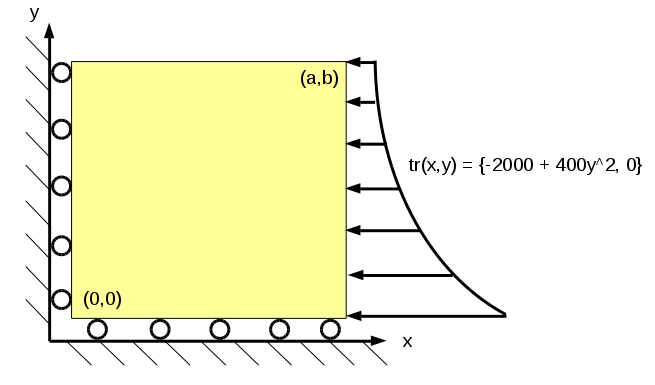
\includegraphics[height = 8cm ]{quadratic_traction}}};
    \caption{Rectangular domain with $a=2$ and $b=2$ units. The left edge has a zero displacement in the x direction boundary condition and a zero displacement in the y direction boundary condition on the bottom edge}
\centering
\end{figure}

\begin{figure}
    \makebox[\textwidth][c]{\adjustbox{trim= {0} {0.20\height} {0} {0.20\height}, clip}{\includegraphics[width = \textwidth ]{convergence_rate}}}
    \caption{Convergence for first and second order finite elements. Substantial inaccuracies that appear as the number of degrees of freedom increase are addressed in the next section.}
\centering
\end{figure}

Before numerical errors appear in the solutions as $h$ gets smaller we do see the expected order of convergence for the different mesh element shape functions. The linear quads and triangles show second order convergence, and the quadratic elements show third order convergence. The increase in error as $h$ further decreases will be discussed in section 4.

\pagebreak
%%=================================================================
\subsection{No Displacement Boundary Conditions, No Tractions}
\FloatBarrier

\begin{figure}
    \makebox[\textwidth][c]{\adjustbox{trim= {0.} {0} {0} {0}, clip}{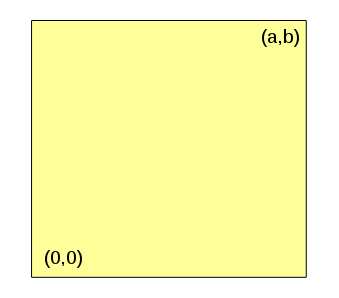
\includegraphics[height = 8cm ]{zero_zero}}};
    \caption{Test boundary value problem: $a = 2$, $b = 2$, $E = 10^8$ and $\nu = 0.35$}
\centering
\end{figure}

With zero constraints and zero tractions, the zero vector is the trivial solution to the linear system. A robust code will properly handle this condition. While other test sections will have a visualization of the displacement solution, the solution to this test is more easily verified numerically in a unit test. Only one mesh solution is shown for reference.

\begin{figure}
    \makebox[\textwidth][c]{\adjustbox{trim= {0.1\width} {0.0\height} {0} {0.0\height}, clip}{\includegraphics[width = \textwidth ]{zero_zero_quad_serendipity}}};
    \caption{Serendipity quadrilateral mesh for a 2 unit by 2 unit rectangular plane shown with displacement scaled by $50,000$ times. The displacement is zero for the entire mesh.}
\centering
\end{figure}

\FloatBarrier
%%=================================================================
\subsection{Some Boundary Constraints, Constant Traction}
\label{subsec:simple_traction}
\FloatBarrier

\begin{figure}
    \makebox[\textwidth][c]{\adjustbox{trim= {0.} {0} {0} {0}, clip}{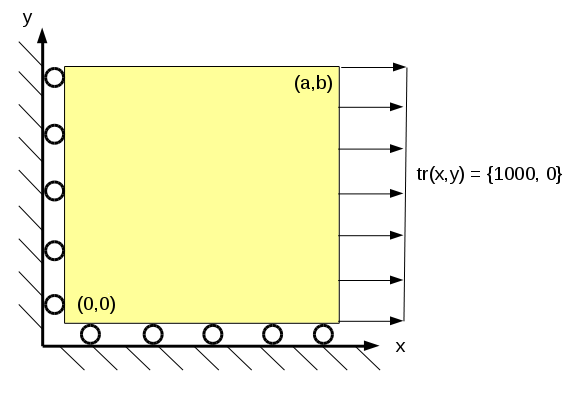
\includegraphics[height = 8cm ]{linear_traction}}};
    \caption{Test boundary value problem: $a = 2$, $b = 2$, $E = 10^8$ and $\nu = 0.35$}
\centering
\end{figure}


\begin{figure}
    \makebox[\textwidth][c]{\adjustbox{trim= {0.1\width} {0.0\height} {0} {0.0\height}, clip}{\includegraphics[width = \textwidth ]{constant_traction_linear_quad}}};
    \caption{Linear quadrilateral mesh for a 2 unit by 2 unit rectangular plane shown with displacement scaled by $50,000$ times}
\centering
\end{figure}

\begin{figure}
    \makebox[\textwidth][c]{\adjustbox{trim= {0.1\width} {0.0\height} {0} {0.0\height}, clip}{\includegraphics[width = \textwidth ]{constant_traction_linear_tri}}};
    \caption{Linear triangle mesh for a 2 unit by 2 unit rectangular plane shown with displacement scaled by $50,000$ times}
\centering
\end{figure}

\begin{figure}
    \makebox[\textwidth][c]{\adjustbox{trim= {0.1\width} {0.0\height} {0} {0.0\height}, clip}{\includegraphics[width = \textwidth ]{constant_traction_quad_quad}}};
    \caption{Quadratic quadrilateral mesh for a 2 unit by 2 unit rectangular plane shown with displacement scaled by $50,000$ times}
\centering
\end{figure}


\begin{figure}
    \makebox[\textwidth][c]{\adjustbox{trim= {0.1\width} {0.0\height} {0} {0.0\height}, clip}{\includegraphics[width = \textwidth ]{constant_traction_serendipity_quad}}};
    \caption{Serendipity mesh for a 2 unit by 2 unit rectangular plane shown with displacement scaled by $50,000$ times}
\centering
\end{figure}

\FloatBarrier
%%=================================================================
\subsection{Some Boundary Constraints,  Quadratic Traction}
\FloatBarrier

\begin{figure}
    \makebox[\textwidth][c]{\adjustbox{trim= {0.} {0} {0} {0}, clip}{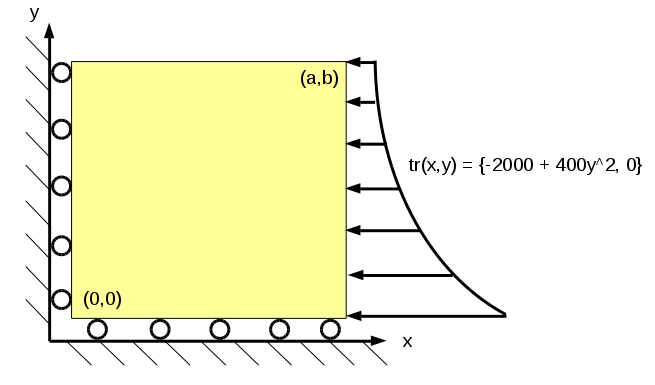
\includegraphics[height = 8cm ]{quadratic_traction}}};
    \caption{Test boundary value problem: $a = 2$, $b = 2$, $E = 10^8$ and $\nu = 0.35$}
\centering
\end{figure}

\begin{figure}
    \makebox[\textwidth][c]{\adjustbox{trim= {0.1\width} {0.0\height} {0} {0.0\height}, clip}{\includegraphics[width = \textwidth ]{quad_traction_linear_quad}}};
    \caption{Linear quadrilateral mesh for a 2 unit by 2 unit rectangular plane shown with displacement scaled by $50,000$ times}
\centering
\end{figure}

\begin{figure}
    \makebox[\textwidth][c]{\adjustbox{trim= {0.1\width} {0.0\height} {0} {0.0\height}, clip}{\includegraphics[width = \textwidth ]{quad_traction_linear_tri}}};
    \caption{Linear triangle mesh for a 2 unit by 2 unit rectangular plane shown with displacement scaled by $50,000$ times}
\centering
\end{figure}

\begin{figure}
    \makebox[\textwidth][c]{\adjustbox{trim= {0.1\width} {0.0\height} {0} {0.0\height}, clip}{\includegraphics[width = \textwidth ]{quad_traction_quad_quad}}};
    \caption{Quadratic quadrilateral mesh for a 2 unit by 2 unit rectangular plane shown with displacement scaled by $50,000$ times}
\centering
\end{figure}


\begin{figure}
    \makebox[\textwidth][c]{\adjustbox{trim= {0.1\width} {0.0\height} {0} {0.0\height}, clip}{\includegraphics[width = \textwidth ]{quad_traction_serendipity_quad}}};
    \caption{Serendipity mesh for a 2 unit by 2 unit rectangular plane shown with displacement scaled by $50,000$ times}
\centering
\end{figure}

\FloatBarrier
%%=================================================================
\subsection{Some Boundary Constraints, Constant Body Force}
\FloatBarrier

\begin{figure}
    \makebox[\textwidth][c]{\adjustbox{trim= {0.} {0} {0} {0}, clip}{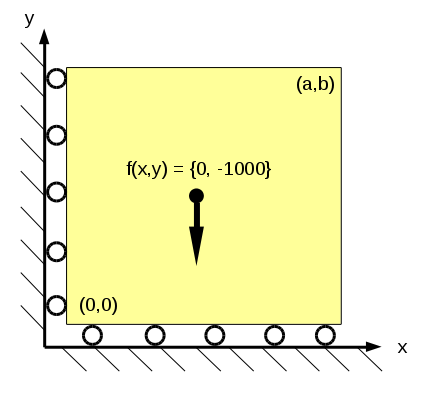
\includegraphics[height = 8cm ]{constant_body}}};
    \caption{Test boundary value problem: $a = 2$, $b = 1$, $E = 10^8$ and $\nu = 0.35$}
\centering
\end{figure}

\begin{figure}
    \makebox[\textwidth][c]{\adjustbox{trim= {0.1\width} {0.10\height} {0} {0.25\height}, clip}{\includegraphics[width = \textwidth ]{gravity_linear_quad}}};
    \caption{Linear quadrilateral mesh for a 2 unit by 1 unit rectangular plane shown with displacement scaled by $50,000$ times}
\centering
\end{figure}

\begin{figure}
    \makebox[\textwidth][c]{\adjustbox{trim= {0.1\width} {0.10\height} {0} {0.25\height}, clip}{\includegraphics[width = \textwidth ]{gravity_linear_tri}}};
    \caption{Linear triangle mesh for a 2 unit by 1 unit rectangular plane shown with displacement scaled by $50,000$ times}
\centering
\end{figure}

\begin{figure}
    \makebox[\textwidth][c]{\adjustbox{trim= {0.1\width} {0.10\height} {0} {0.25\height}, clip}{\includegraphics[width = \textwidth ]{gravity_quadratic_quad}}};
    \caption{Quadratic quadrilateral mesh for a 2 unit by 1 unit rectangular plane shown with displacement scaled by $50,000$ times}
\centering
\end{figure}


% \begin{figure}
%     \makebox[\textwidth][c]{\adjustbox{trim= {0.1\width} {0.10\height} {0} {0.25\height}, clip}{\includegraphics[width = \textwidth ]{gravity_linear_quad}}};
%     \caption{Quadratic triangle mesh for a 2 unit by 1 unit rectangular plane shown with displacement scaled by $50,000$ times}
% \centering
% \end{figure}

\begin{figure}
    \makebox[\textwidth][c]{\adjustbox{trim= {0.1\width} {0.10\height} {0} {0.25\height}, clip}{\includegraphics[width = \textwidth ]{gravity_serendipity_quad}}};
    \caption{Serendipity mesh for a 2 unit by 1 unit rectangular plane shown with displacement scaled by $50,000$ times}
\centering
\end{figure}


\FloatBarrier

%%=================================================================
\subsection{Some Boundary Constraints, Linear Body Force}
\FloatBarrier

\begin{figure}
    \makebox[\textwidth][c]{\adjustbox{trim= {0.} {0} {0} {0}, clip}{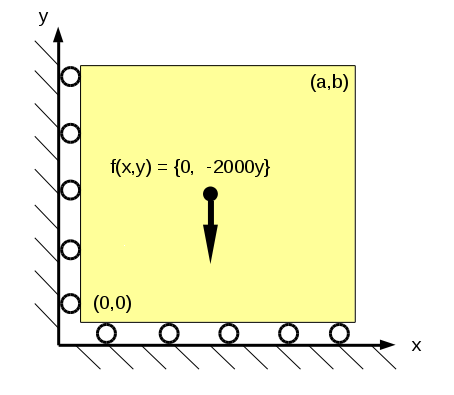
\includegraphics[height = 8cm ]{linear_body}}};
    \caption{Test boundary value problem: $a = 2$, $b = 2$, $E = 10^8$ and $\nu = 0.35$}
\centering
\end{figure}

\begin{figure}
    \makebox[\textwidth][c]{\adjustbox{trim= {0.1\width} {0.0\height} {0} {0.0\height}, clip}{\includegraphics[width = \textwidth ]{linear_body_linear_quad}}};
    \caption{Linear quadrilateral mesh for a 2 unit by 2 unit rectangular plane shown with displacement scaled by $50,000$ times}
\centering
\end{figure}

\begin{figure}
    \makebox[\textwidth][c]{\adjustbox{trim= {0.1\width} {0.0\height} {0} {0.0\height}, clip}{\includegraphics[width = \textwidth ]{linear_body_linear_tri}}};
    \caption{Linear triangle mesh for a 2 unit by 2 unit rectangular plane shown with displacement scaled by $50,000$ times}
\centering
\end{figure}

\begin{figure}
    \makebox[\textwidth][c]{\adjustbox{trim= {0.1\width} {0.0\height} {0} {0.0\height}, clip}{\includegraphics[width = \textwidth ]{linear_body_quad_quad}}};
    \caption{Quadratic quadrilateral mesh for a 2 unit by 1 unit rectangular plane shown with displacement scaled by $50,000$ times}
\centering
\end{figure}


\begin{figure}
    \makebox[\textwidth][c]{\adjustbox{trim= {0.1\width} {0.0\height} {0} {0.0\height}, clip}{\includegraphics[width = \textwidth ]{linear_body_serendipity_quad}}};
    \caption{Serendipity mesh for a 2 unit by 2 unit rectangular plane shown with displacement scaled by $50,000$ times}
\centering
\end{figure}


\FloatBarrier

\section{Notable Bugs}

\FloatBarrier

\begin{figure}
    \makebox[\textwidth][c]{\adjustbox{trim= {0} {0.2\height} {0} {0.15\height}, clip}{\includegraphics[width = 0.8\textwidth ]{smaller_h_constant_force}}};
    \caption{Convergence of meshes of same geometrical problem with different types of mesh elements. $E = 8*10^8$ and $\nu = 0.35$}
\centering
\end{figure}
We change the size of the domain of the boundary value problem to detect any type of rounding errors or loss of precision from underflow. Using a domain that is an order of magnitude larger that the first problem, the error with the strain energy does not change noticeably.
\begin{figure}
    \makebox[\textwidth][c]{\adjustbox{trim= {0} {0.2\height} {0} {0.15\height}, clip}{\includegraphics[width = 0.8\textwidth ]{smaller_h_constant_force_20x20}}};
    \caption{Convergence of meshes of same geometrical problem with different types of mesh elements. $E = 8*10^8$ and $\nu = 0.35$}
\centering
\end{figure}


\begin{figure}
    \makebox[\textwidth][c]{\adjustbox{trim= {0} {0.2\height} {0} {0.15\height}, clip}{\includegraphics[width = 0.8\textwidth ]{difference_between_10_80_linear_tri_gravity}}};
    \caption{Difference in deformation solution between a 10x10 mesh and a 80x80 mesh for linear triangle elements. $E = 8*10^8$ and $\nu = 0.35$}
\centering
\end{figure}
\FloatBarrier
We check to see if this could be an issue with the chosen solver finding a close enough solution to the systems of equations. We are using an inexact solver, so this scenario is plausible. Plotting the strain energy against the degrees of freedom will reveal any dependence on solver inaccuracies.
\FloatBarrier
\begin{figure}
    \makebox[\textwidth][c]{\adjustbox{trim= {0} {0.2\height} {0} {0.15\height}, clip}{\includegraphics[width = 0.8\textwidth ]{error_vs_dofs}}};
    \caption{Strain energy plotted vs degrees of freedom in the linear system passed to the solver which has fixed degrees of freedom from boundary constraints already reduced}
\centering
\end{figure}
\FloatBarrier
From the figure we see two different behaviors for different mesh elements. The quadrilateral elements all show similar degradation in the accuracy of the solution at around 15 thousand degrees of freedom. For triangular elements the loss in accuracy does not appear to have a common break point. This indicates that there is a separate bug with the implementation of triangular elements. Implementing the third order Lagrange shape functions would help test this hypothesis. Right now there are only two data points for the behavior of triangular elements, which makes pattern fitting more difficult. Checking the norm of the solution produced by the solver $||Kd - F||$ would also give more information about potential implementation errors or misuse of PETSc solvers.


\FloatBarrier
%%=================================================================
\subsection{Non Zero Dirichlet Boundary Conditions}
Non zero essential boundary conditions are incorrectly implemented. It appears that there
is an array indexing bug when converting from global degrees of freedom to the local degrees of freedom of the linear system passed to the solver. Each of the different mesh types has a different displacement which changes per run of the software, indicating that a buffer may be uninitialized. Notice that only a few elements seem warped, while the majority appear to correctly deflect given the influence of the few corrupt elements.
\FloatBarrier

\begin{figure}
    \makebox[\textwidth][c]{\adjustbox{trim= {0.} {0} {0} {0}, clip}{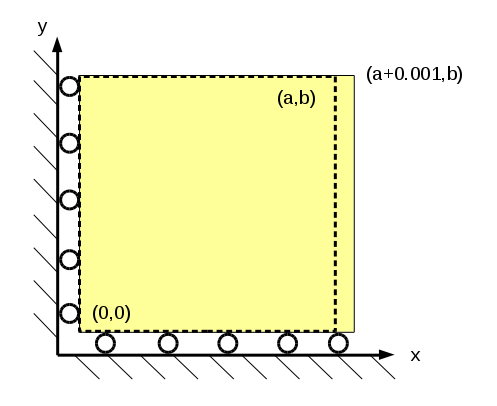
\includegraphics[height = 8cm ]{nonzero_dirichlet}}};
    \caption{Test boundary value problem: $a = 2$, $b = 2$, $E = 10^8$ and $\nu = 0.35$}
\centering
\end{figure}

\begin{figure}
    \makebox[\textwidth][c]{\adjustbox{trim= {0.1\width} {0.0\height} {0} {0.0\height}, clip}{\includegraphics[width = \textwidth ]{dirichlet_linear_quad}}};
    \caption{Linear quadrilateral mesh for a 2 unit by 2 unit rectangular plane shown with displacement scaled by $10$ times}
\centering
\end{figure}

\begin{figure}
    \makebox[\textwidth][c]{\adjustbox{trim= {0.1\width} {0.0\height} {0} {0.0\height}, clip}{\includegraphics[width = \textwidth ]{dirichlet_linear_tri}}};
    \caption{Linear triangle mesh for a 2 unit by 2 unit rectangular plane shown with displacement scaled by $10$ times}
\centering
\end{figure}

\begin{figure}
    \makebox[\textwidth][c]{\adjustbox{trim= {0.1\width} {0.0\height} {0} {0.0\height}, clip}{\includegraphics[width = \textwidth ]{dirichlet_quad_quad}}};
    \caption{Quadratic quadrilateral mesh for a 2 unit by 1 unit rectangular plane shown with displacement scaled by $10$ times}
\centering
\end{figure}


\begin{figure}
    \makebox[\textwidth][c]{\adjustbox{trim= {0.1\width} {0.0\height} {0} {0.0\height}, clip}{\includegraphics[width = \textwidth ]{dirichlet_serendipity_quad}}};
    \caption{Serendipity mesh for a 2 unit by 2 unit rectangular plane shown with displacement unscaled}
\centering
\end{figure}

\FloatBarrier

\section{Pseudo code}

Not completed

% \begin{algorithm}
% \begin{algorithmic}

% \Procedure{Foo}{bar}
%     \State Foo
% \EndProcedure

% \end{algorithmic}
% \end{algorithm}

% \begin{algorithm}
% \begin{algorithmic}

% \Procedure{IntegrateStiffness}{element, weight, dV}
%     \State n\_local\_dofs $\gets$ NDIM $*$ countElementNodes(element) \Comment{2} 
%     \State K\_element $\gets$ Matrix< n\_local\_dofs, n\_local\_dofs >
%     \ForAll{integration\_point \textbf{on} element}
%         \State gradShape $\gets$ getShapeGradient(integration\_point)
%         \Comment Construct
%         \ForAll{node \textbf{in} element}
%             \State B[node\_index] $\gets$ $ \left[  \right]$
%         \EndFor
%     \EndFor
% \EndProcedure

% \end{algorithmic}
% \end{algorithm}



% \begin{figure}
%     \makebox[\textwidth][c]{\adjustbox{trim= {0.15\width} {0} {0.15\width} {0}, clip}{\includegraphics[width = \textwidth ]{part1_pre_migr}}};
%     \caption{Partition 1 surface before region migration}
% \centering


\section{Source Code Listings}

\lstset{linewidth = 16cm, xrightmargin = 0cm}
\lstlistoflistings
%includes
\lstinputlisting[caption = {Algebraic System container class}]{../inc/AlgebraicSystem.h}
\lstinputlisting[caption = {Elastic Analysis Class}]{../inc/ElasticAnalysis2D.h}
\lstinputlisting[caption = {Abstract Base FE Analysis class}]{../inc/FEAnalysis.h}
\lstinputlisting[caption = {Force Contributor}]{../inc/ForceContributor2D.h}
\lstinputlisting[caption = {Mesh Builder helper class}]{../inc/MeshBuilder.h}
\lstinputlisting[caption = {Adjacency reordering routine}]{../inc/MeshAdjReorder.h}
\lstinputlisting[caption = {Stiffness Constributor}]{../inc/StiffnessContributor2D.h}
\lstinputlisting[caption = {Recover Secondary Variables}]{../inc/RecoverAtIntegrationPoints.h}

%sources
\lstinputlisting[caption = {Algebraic System implementation}]{../src/AlgebraicSystem.cc}
\lstinputlisting[caption = {Elastic Analysis implementation}]{../src/ElasticAnalysis2D.cc}
\lstinputlisting[caption = {Force Contributor implementation}]{../src/ForceContributor2D.cc}

\lstinputlisting[caption = {Stiffness contributor implementation}]{../src/StiffnessContributor2D.cc}
\lstinputlisting[caption = {Geometry Mapping Implementation}]{../src/GeometryMappings.cc}
\lstinputlisting[caption = {Mesh Adjacency reordering implementation}]{../src/MeshAdjReorder.cc}
\lstinputlisting[caption = {Mesh builder scripts}]{../src/MeshBuilder.cc}

%tests
\lstinputlisting[caption = {Test Driver}]{../src/mpi_and_petsc_gtest_main.cc}
%Mesh builder unittests are all empty right now and probably wont meaningfully change
%\lstinputlisting[caption = {Mesh builder unittests}]{../src/MeshBuilder_unittest.cc}
\lstinputlisting[caption = {Measures convergence of mesh elements}]{../src/Convergence_test.cc}
\lstinputlisting[caption = {Abstract common testing setup code}]{../inc/TestingUtilityFunctions.h}
\lstinputlisting[caption = {Algebraic System tests}]{../src/AlgebraicSystem_unittest.cc}
\lstinputlisting[caption = {Test node mapping functions}]{../src/ShapeFunctionOrdering_unittest.cc}
\lstinputlisting[caption = {Test mesh generation scripts}]{../src/SimpleRectMesh_unittest.cc}
\lstinputlisting[caption = {Geometry Mapping tests}]{../src/GeometryMappings_unittest.cc}

%build files
\lstinputlisting[caption = {configuration file}]{../config.mk}
\lstinputlisting[caption = {Makefile}]{../Makefile}
\lstinputlisting[caption = {Travis CI}] {../../.travis.yml}


\end{document}
